\chapter{Une architecture d'habitats intelligents modernisée}
\label{chap:5}

\section{Introduction}

Il a été vu, dans les chapitres précédents qu'au fil des ans, diverses architectures de maisons intelligentes ont été proposées et mises en place au sein de laboratoires ou dans de réelles habitations pour mener des activités de recherche \citep{DJCook2003,Helal2005,Giroux2009,Cook2013,Bouchard2014,Lago2017,Plantevin2018}. Ces travaux se sont particulièrement intéressés à l'utilisation de capteurs, d'effecteurs et de techniques d'apprentissage machine pour la mise en application de l'\acl{IAm} comme méthode empirique afin de soutenir l'autonomie des personnes âgées et le suivi de la santé. Cependant, bien que chacun de ces travaux se distingue des autres, tous proposent différentes méthodes pour résoudre le problème principal qu'il cherchent à résoudre demeure la reconnaissance d'activités. Les avantages et les inconvénients de chaque architecture d'habitats intelligents ont déjà été discutés dans cette thèse et le principal problème qui a été identifié réside dans le manque de fiabilité et l'évolutivité de ces implémentations. En effet, la plupart des architectures admettent au moins un point de défaillance unique (\acl{SPOF} ou \acs{SPOF}) principalement à cause de leur implémentation centralisée, ou \og monolithique \fg. Néanmoins, il a aussi été montré que \cite{Plantevin2018} ont adressé cette problématique en introduisant un nouveau type d'architecture basée sur l'utilisation de transducteurs intelligents distribués. Cependant, bien que cette implémentation ait été pensée pour être une architecture de maisons intelligentes prête à l'emploi en situation réelle d'utilisation, sa conception ne semble pas suffisamment adaptée aux environnements de recherche. En effet, la simplicité de mise en place de nouvelles méthodes pour la reconnaissance d'activités et de nouveaux protocoles expérimentaux semble avoir été oubliés dans cette implémentation.

Par ailleurs, dans la comparaison des différentes architectures de maisons intelligentes proposées au chapitre \ref{chap:2}, le principal inconvénient des solutions existantes qui a été identifié concerne leur manque de flexibilité quant à l'intégration de nouveaux matériels et plus spécifiquement, les \textit{wearable devices}. En effet, pour réaliser la reconnaissance d'activités, la plupart des méthodes proposées avec ses dispositifs sont des applications complètes. La plupart du temps, les différents processus qui composent la reconnaissance sont encapsulés au sein d'un unique composant logiciel immuable. Il devient donc difficile de les modifier. De plus, le fait de disposer d'une unique application ne favorise pas la réutilisation de certains mécanismes communs à plusieurs méthodes. Ceux-ci doivent donc généralement être soit développés à nouveau, soit adaptés afin de pouvoir supporter des modifications dans la méthode proposée. De plus, l'exploitation de ce genre d'application \og prête à l'emploi \fg est, la plupart du temps, complexifiée. En effet, selon les dépendances, le langage de programmation et la plateforme, elles peuvent être difficiles à adapter et à déployer d'un environnement à un autre (\textit{p. ex.} entre deux laboratoires de recherche différents).

Ainsi, ce travail présente un autre type d'architecture de maisons intelligentes qui se veut fiable et évolutive dont l'implémentation est inspirée des architectures de \textit{cloud} privées sur site. Cette architecture vise à résoudre la plupart des problèmes identifiés au sein des implémentations précédemment proposées sans qu'il soit nécessaire de remplacer leur structure au complet. En effet, l'implémentation présentée dans ce chapitre a été pensée pour à la fois être déployée en l'état, ou pour s'intégrer aux architectures existantes, remplaçant ainsi les entités centrales des architectures monolithiques. L'objectif principal de cette implémentation est alors de pouvoir y déployer facilement de nouveaux composants logiciels expérimentaux indépendamment des différences dans leur conception, tant en termes de langages de programmation que de librairies requises ou de plateforme supportées. Ceci dans le but de favoriser l'interopérabilité entre les différents processus, leur réutilisation ainsi que leur mise à l'échelle vis-à-vis de la quantité de ressources requise.

La suite de ce chapitre comporte une première section qui présente en détail l'architecture d'habitats intelligents proposée. Ensuite, les expérimentations sont décrites dans une seconde section. De plus, cette section propose une discussion des observations réalisées. Finalement, dans une dernière partie, une conclusion est dressée quant à ce second travail.

\section{Architecture Proposée}

L'architecture introduite dans ce chapitre a été conçue pour être compatible avec la majorité des architectures de maisons intelligentes présentes dans la littérature. Par conséquent, celle-ci peut être considérée comme une extension du travail proposé par \cite{Plantevin2018}, puisqu'ils ont concentré leurs efforts sur la suppression des \acsp{SPOF} dans le but d'améliorer la fiabilité globale des habitats intelligents existants. Néanmoins, l'idée principale de ce travail est d'aller plus loin dans l'idée de rendre ces architectures plus fiables et plus flexibles. Pour ce faire, ce chapitre présente une implémentation qui repose sur l'utilisation des microservices plutôt qu'une approche monolithique.

\subsection{Microservices}

\begin{figure}[H]
	\centering
	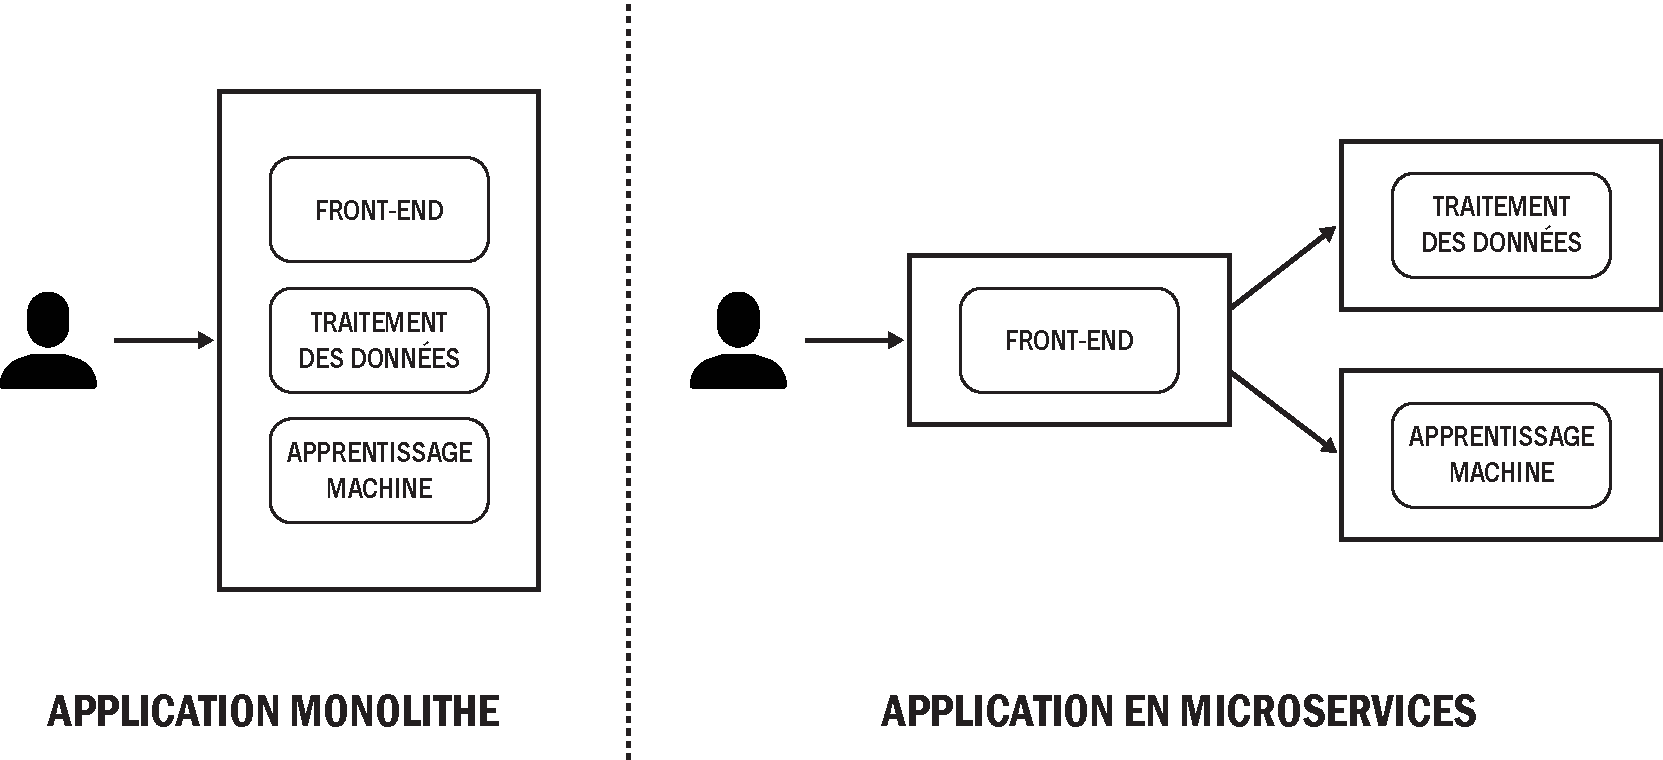
\includegraphics[width=.8\linewidth]{chapter5/mono_micro.pdf}
        \caption{caption}
	\label{fig:mono_micro}
\end{figure}

\begin{figure}[H]
	\centering
	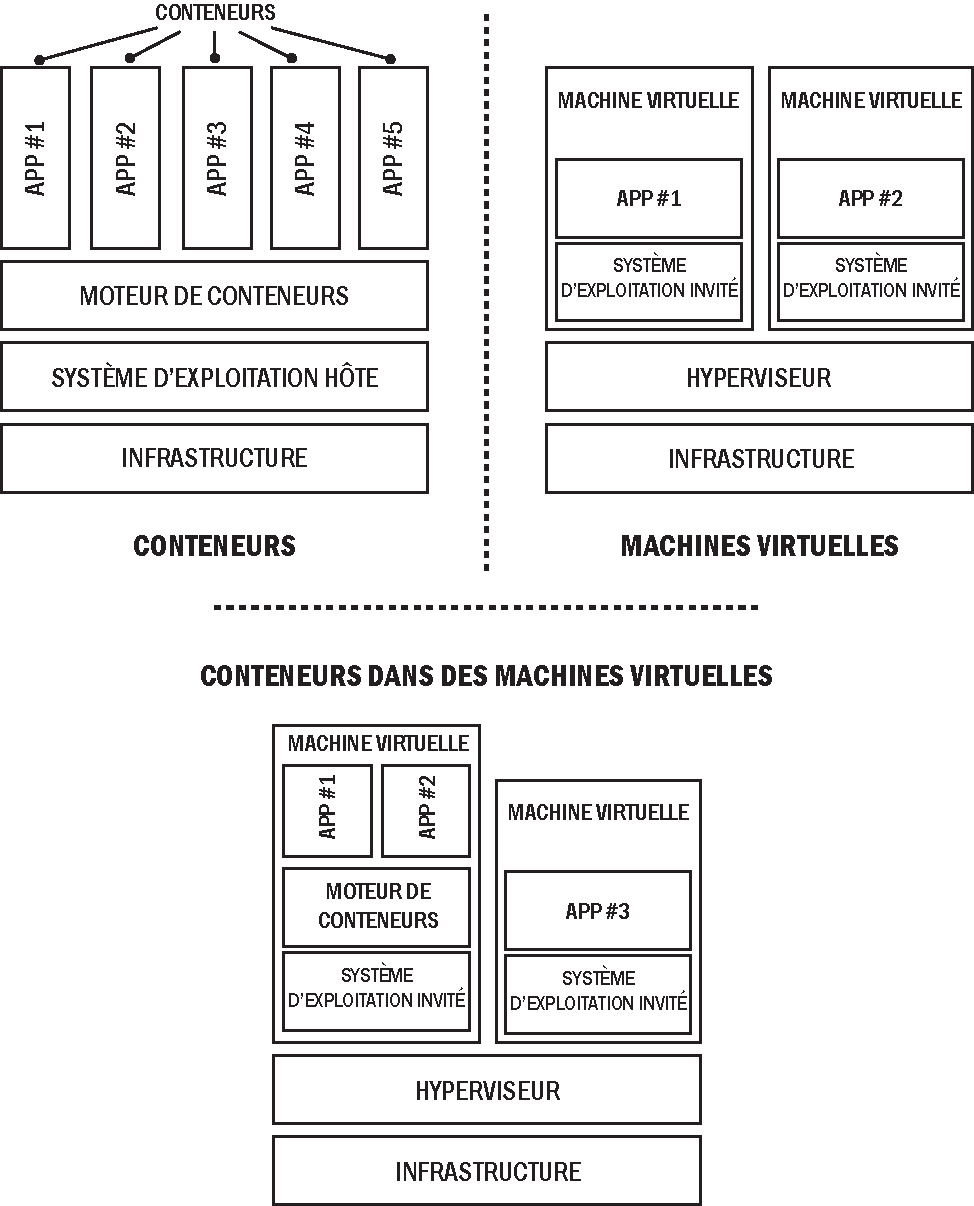
\includegraphics[width=.8\linewidth]{chapter5/containers_vms.pdf}
        \caption{caption}
	\label{fig:containers_vms}
\end{figure}

\subsection{Implémentation}

\begin{figure}[H]
	\centering
	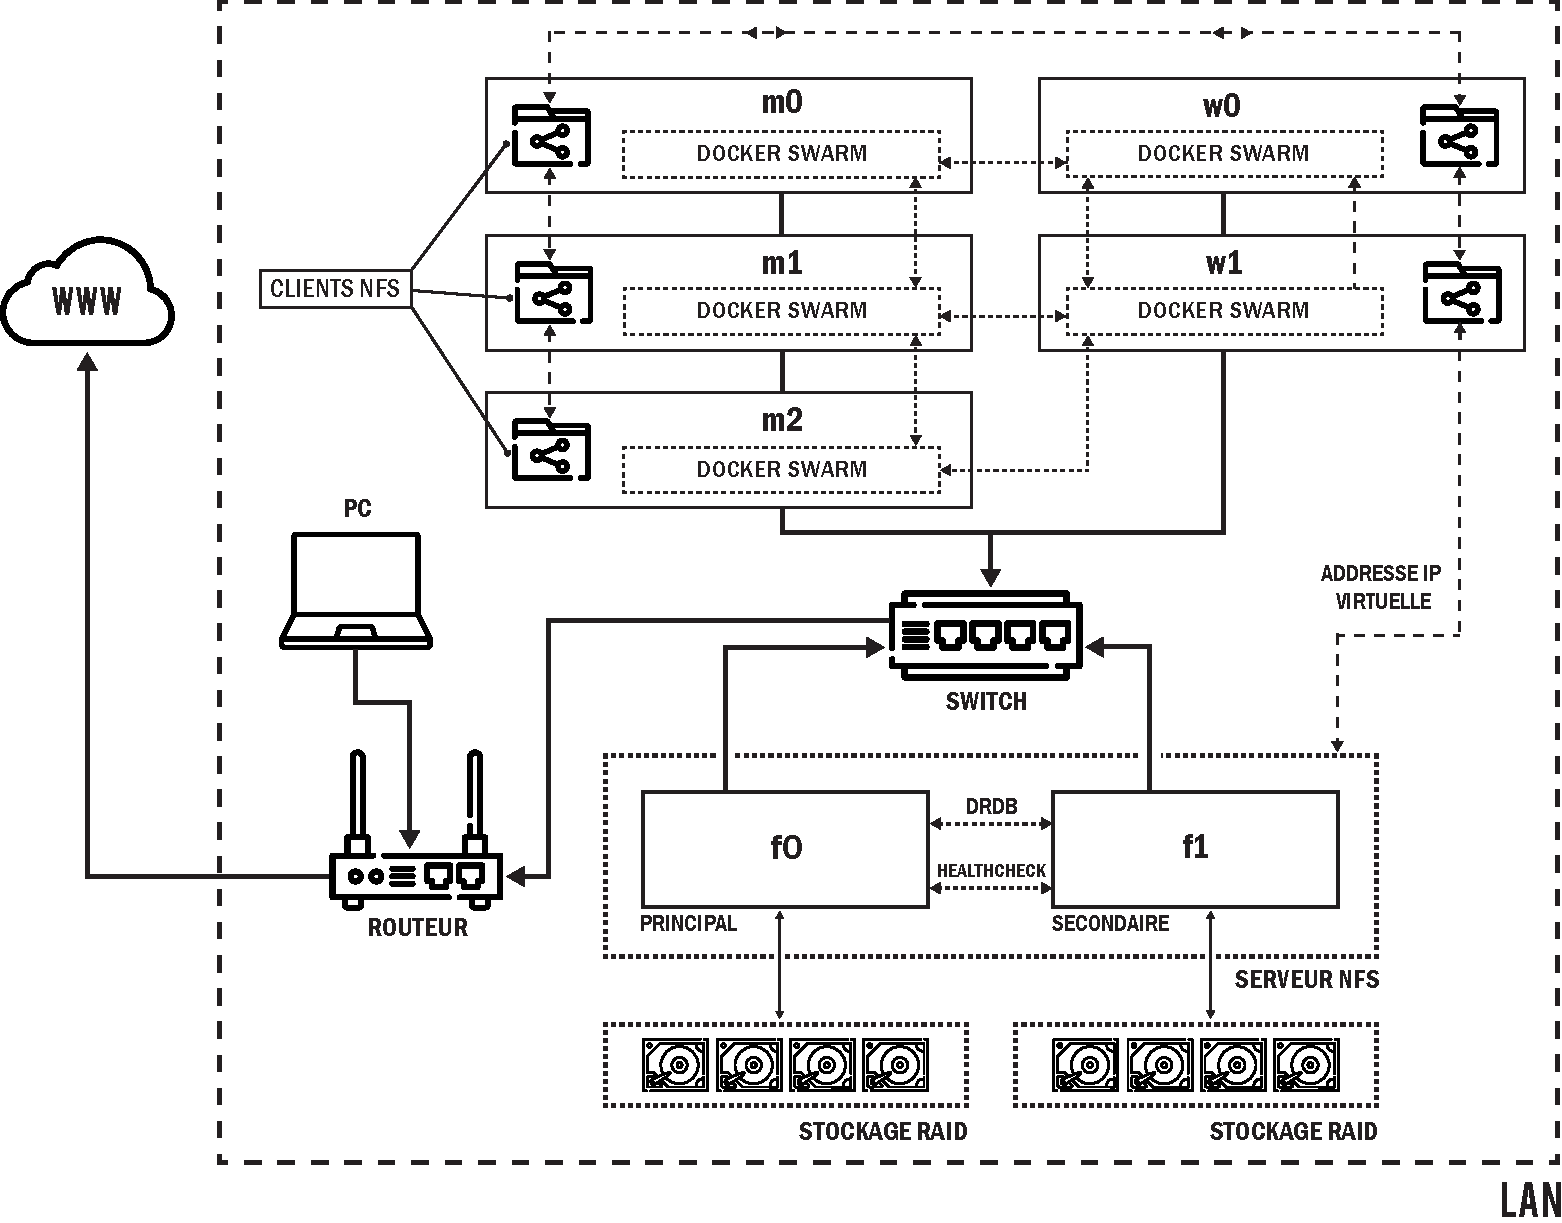
\includegraphics[width=.8\linewidth]{chapter5/proposed_arch.pdf}
        \caption{caption}
	\label{fig:proposed_arch}
\end{figure}

\subsection{Système de fichiers hautement disponible}

\subsection{Orchestration des conteneurs}

\begin{figure}[H]
	\centering
	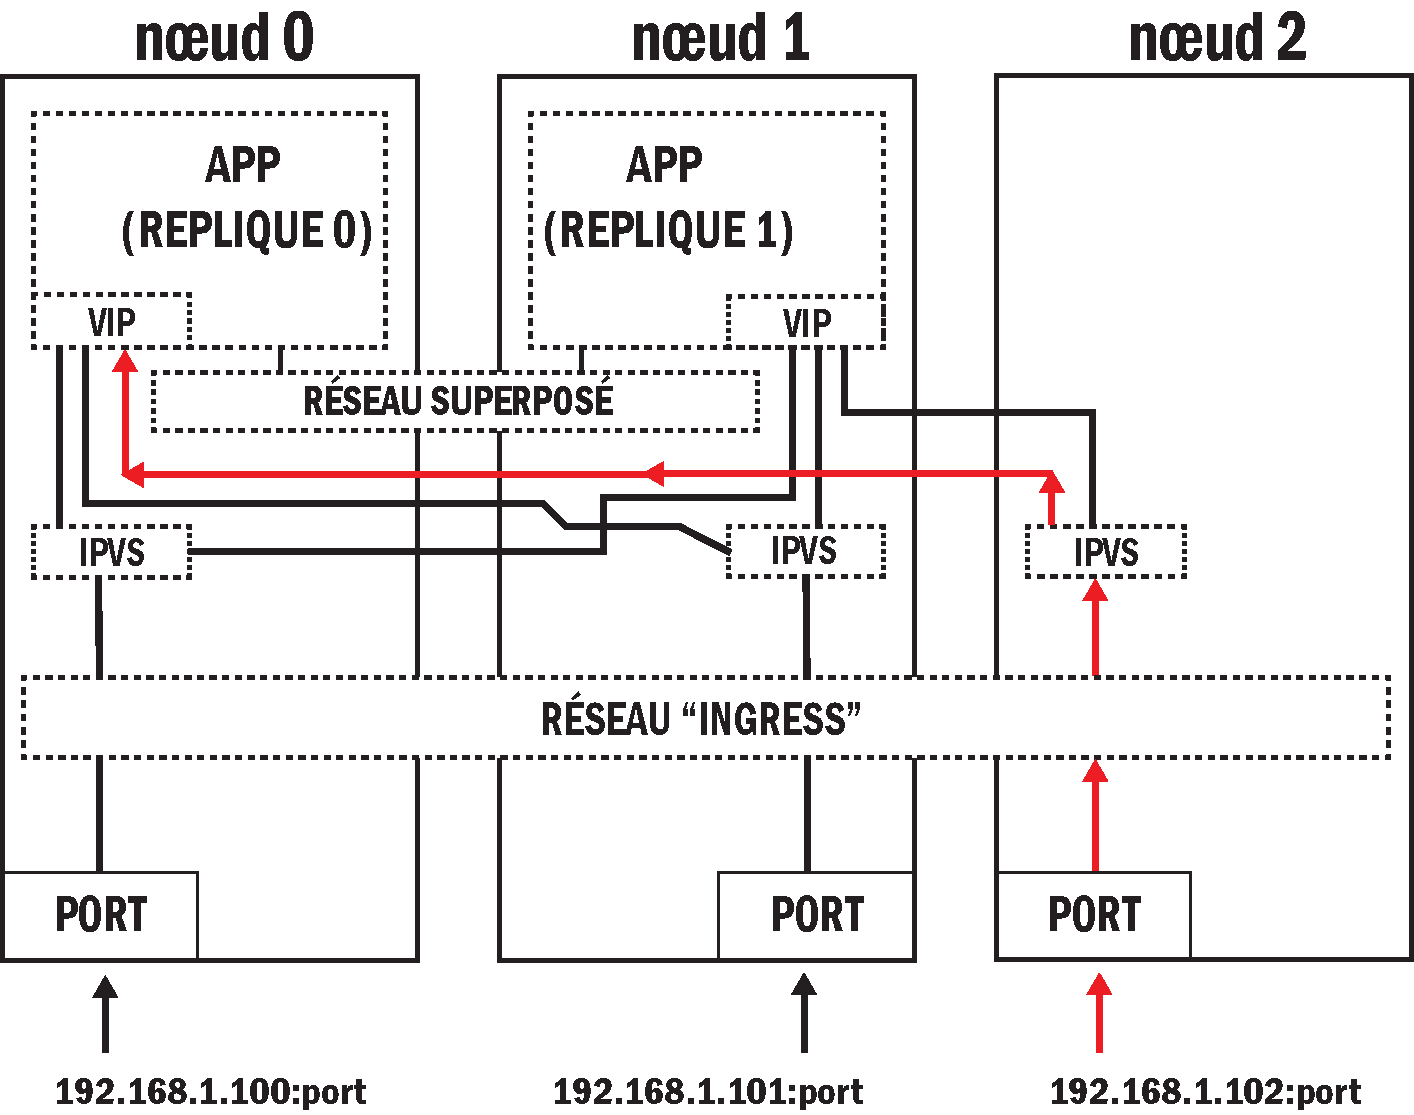
\includegraphics[width=.8\linewidth]{chapter5/swarm_load_balancing.pdf}
        \caption{caption}
	\label{fig:swarm_load_balancing}
\end{figure}

\subsection{Proxy inverse}

\begin{figure}[H]
	\centering
	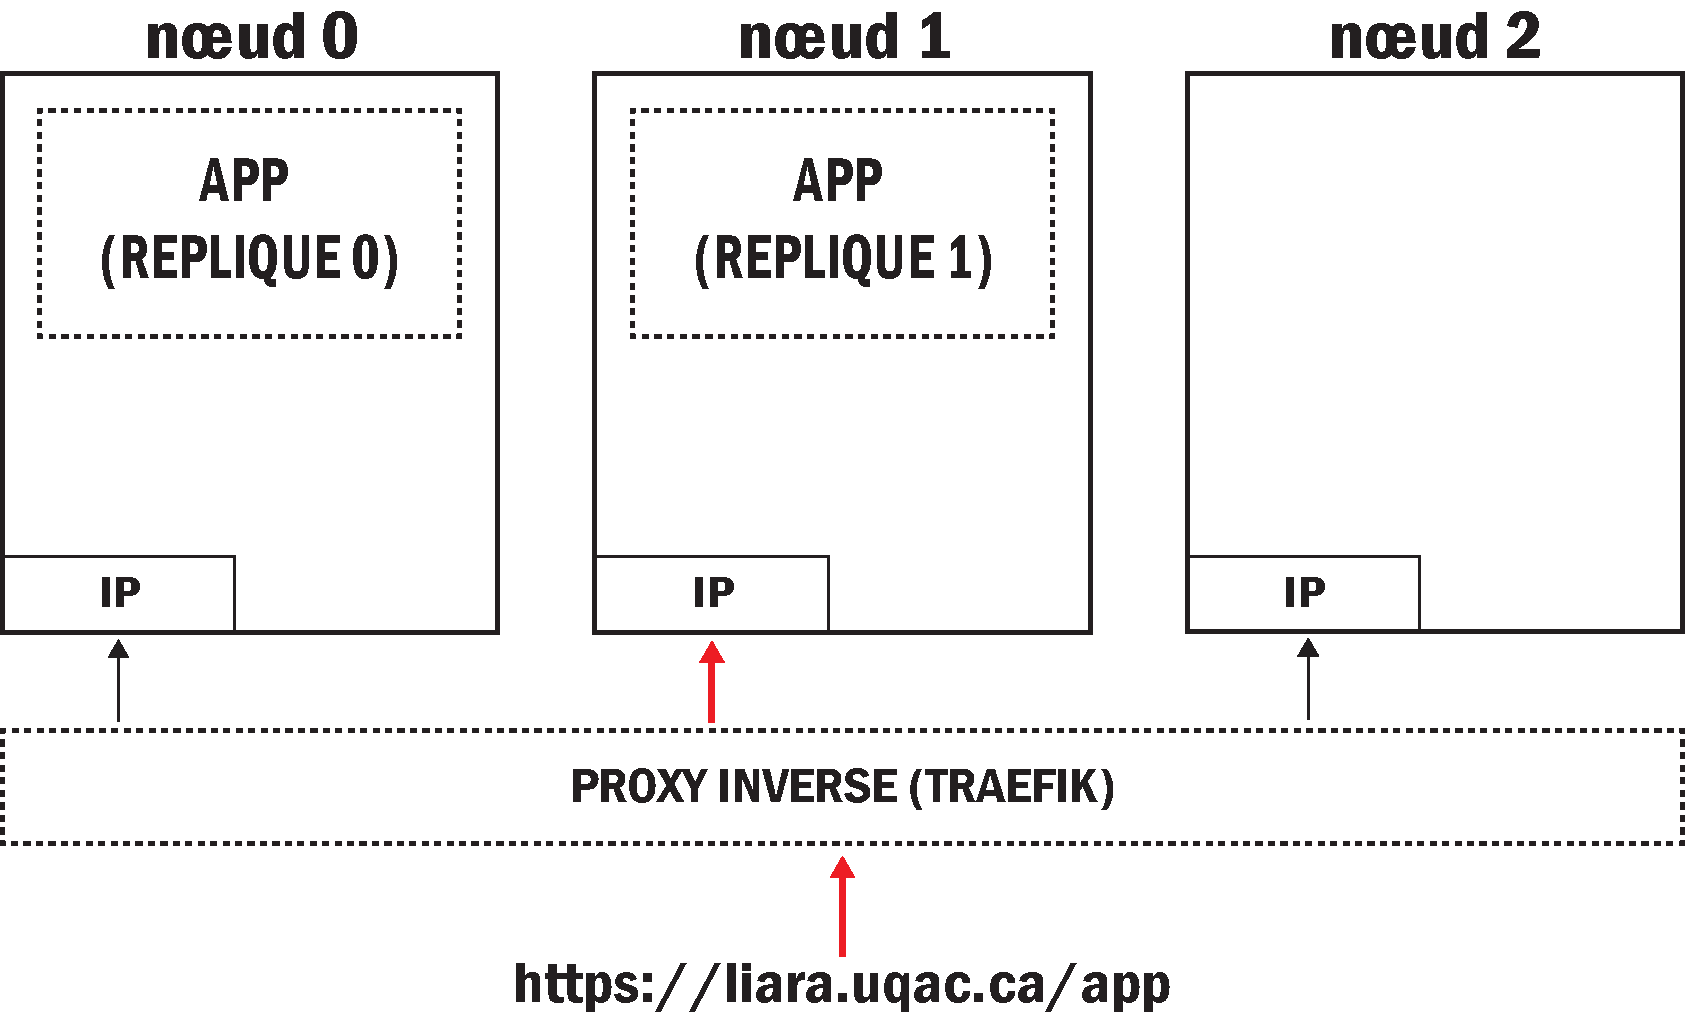
\includegraphics[width=.8\linewidth]{chapter5/arch_reverse_proxy.pdf}
        \caption{caption}
	\label{fig:arch_reverse_proxy}
\end{figure}

\subsection{Gestion du cluster}

\subsection{Base de données répliquée}

\begin{figure}[H]
	\centering
	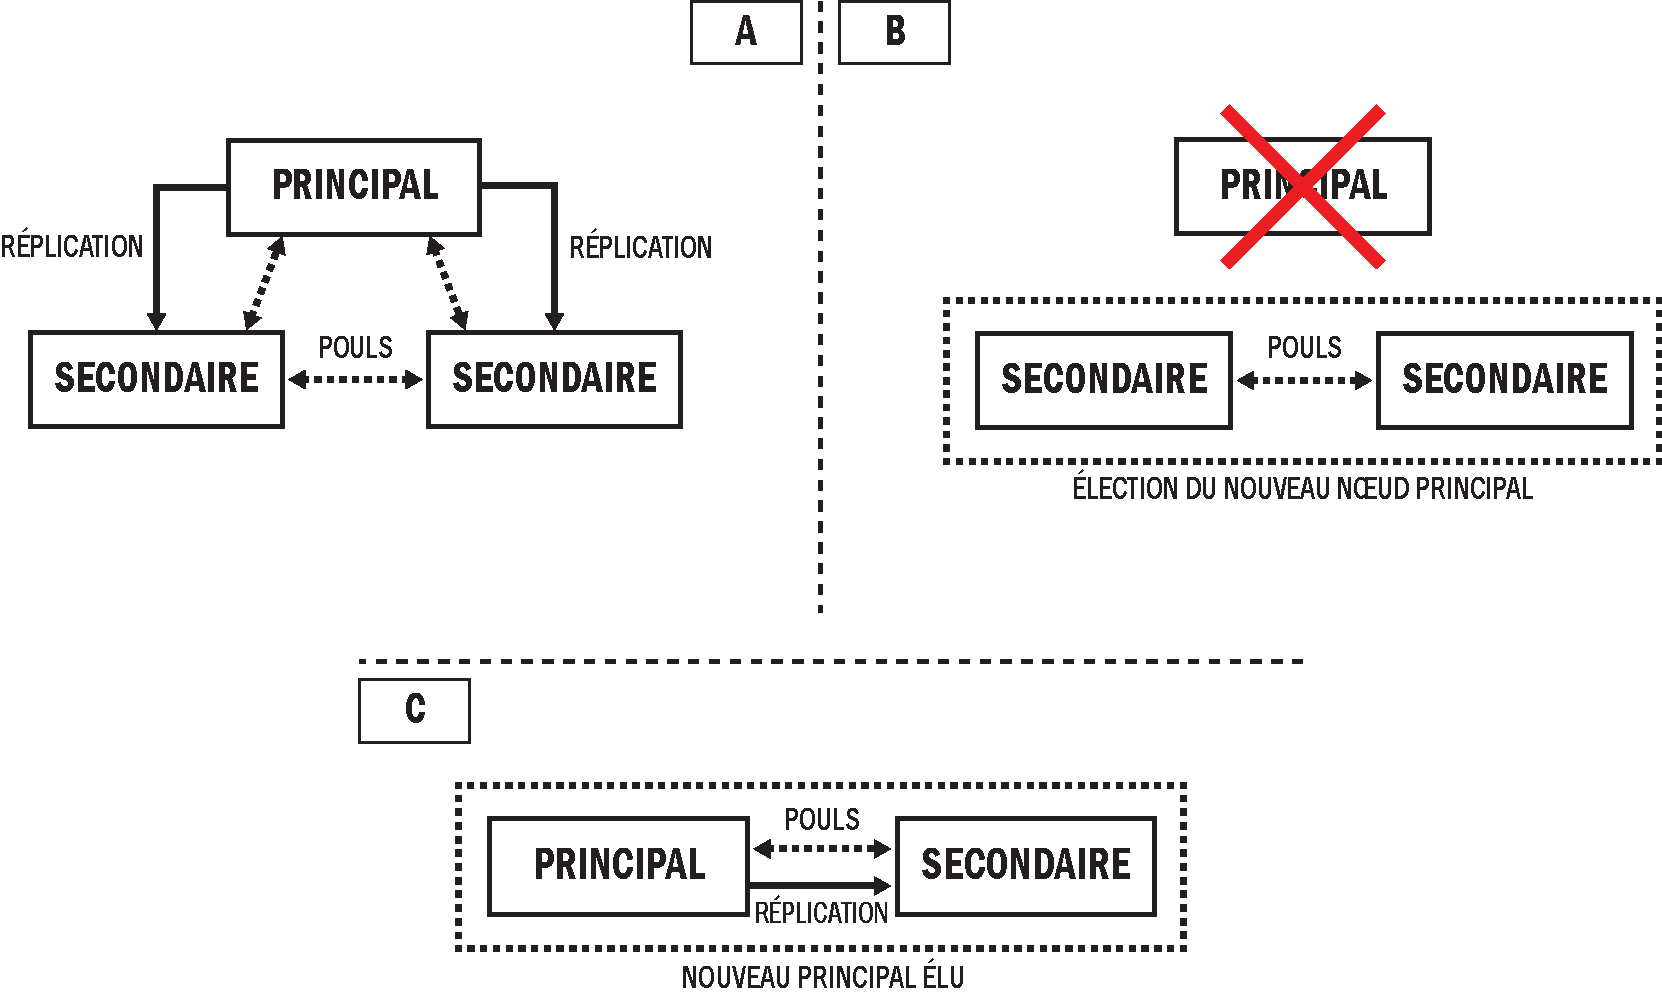
\includegraphics[width=.8\linewidth]{chapter5/mongodb_replication.pdf}
        \caption{caption}
	\label{fig:mongodb_replication}
\end{figure}

\subsection{Dépôt de conteneurs}

\subsection{Organisation des conteneurs}

\begin{figure}[H]
	\centering
	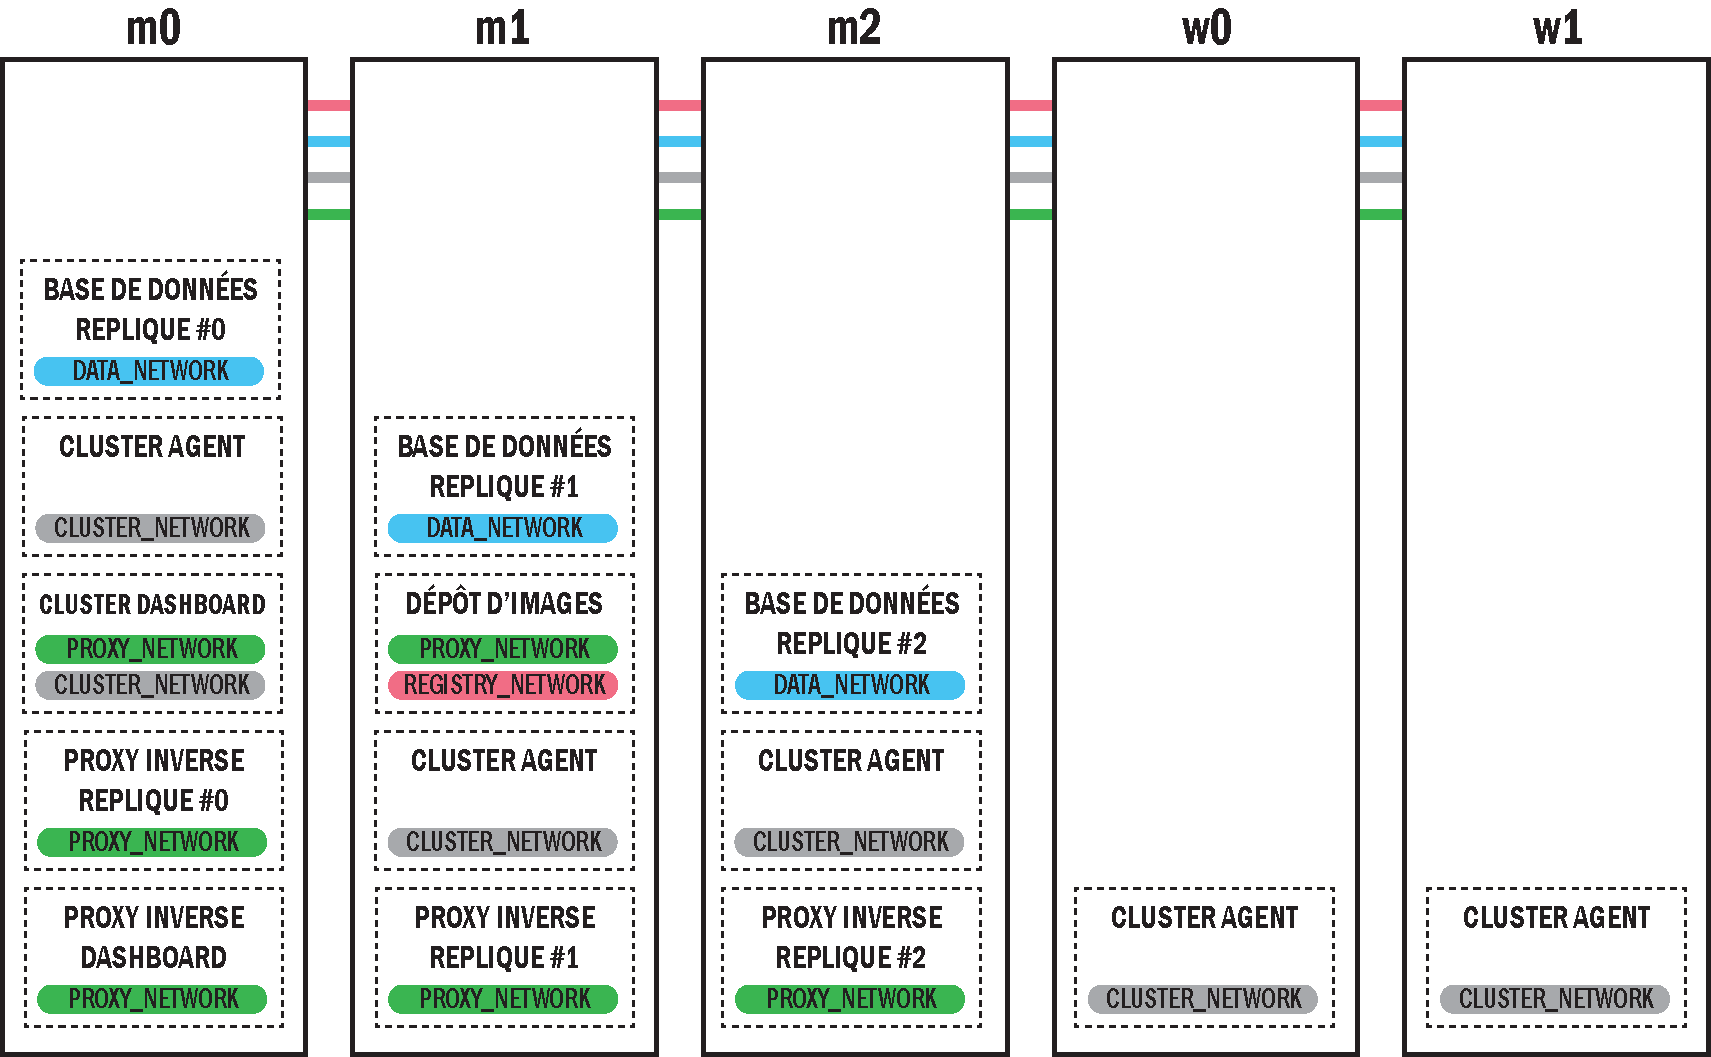
\includegraphics[width=.8\linewidth]{chapter5/containers.pdf}
        \caption{caption}
	\label{fig:containers}
\end{figure}


\section{Experimentations}

\subsection{Installation Matérielle}

\subsection{Haute disponibilité}

\section{Conclusion}